
\chapter{Konzeptionierung einer integrierten Python Anwendung}\label{PythonApp}

Die Basisanforderungen einer integrierten LZ-Verwaltung lassen sich aus den Kapiteln \ref{SoftwareArchitektur} und \ref{Funktionsanalyse} ableiten.

Hinzu kommen die später in Kapitel 5 beschriebenen Funktionen.

Neben den Kriterien Modularität, Erweiterbarkeit und Wartbarkeit ist darüber hinaus wichtig, dass auch Personen,
die bei der ursprünglichen Entwicklung der Software nicht involviert waren, die Software warten und weiterentwickeln können.

Eine saubere Struktur und eine gute Dokumentation der Software ist daher unerlässlich. 
Eine objektorientierte Programmierung bietet sich an, da andere Teile der $\mu$Plant dieses Programmierparadigma nutzen.

Das Programm \glqq Lagerverwaltung 3.0\grqq{} nutzte eine GUI-Klasse als Datenhub und verfügt ansonsten über kein zentrales Datenmodell.
Dadurch entstand ein unübersichtliches Klassenkonstrukt, dass es schwer macht den Datenfluss zu ermitteln.

Zum Beispiel wird anhand der Klassendiagramme deutlich, dass Daten der Modbus Adressen in die \verb|commissionMatrix|
geschrieben werden müssen, weil sie ausschließlich dort zu RAPID Kommandos für den Industrieroboter übersetzt werden.
Wie genau das passiert, lässt sich jedoch anhand des C\# Codes nicht nachvollziehen.

\section{Datenmodellierung}

Um den Anforderungen gerecht zu werden, empfiehlt es sich auf übliche Design Patterns der Softwareentwicklung zu setzen.
Das MVC Konzept sieht vor, dass Daten (Model) und GUI (View) keinerlei Zugriff aufeinander erlauben.
Die Schnittstelle zwischen den Daten und dem Benutzer ist ein Controller, der die Programmlogik implementiert.
Für die Daten gilt, dass sie in einer Objektstruktur modelliert werden und nicht von außerhalb dieser Objekte verändert
werden.

Soll das Datenmodell geändert werden, muss dafür eine öffentliche Methode in dem Modell selbst existieren,
die alle möglichen Fehler behandelt und referenzielle Integrität herstellt, sodass das Datenmodell nach jeder berechtigten
Änderung konsistent bleibt und unberechtigte Änderungen nicht zulässt.

Die drei Klassen in Abb. \ref{fig:figure9} besitzen private Attribute, was durch das \glqq -\grqq{} angedeutet ist.

Dafür besitzen sie öffentliche Methoden ( durch das \glqq +\grqq{} gekennzeichnet), die einerseits die Attribute zurückgeben (get-Methoden) oder einen zu verändernden
Wert übernehmen (set - Methoden).

Werden Listen verwendet, können Objekte mit den with- und without - Methoden hinzugefügt oder entfernt werden.

Ein Objekt der Klasse \verb|Pallet| kann sich also nicht direkt selbst in das entsprechende Feld eines Objekts der Klasse
\verb|Cup| eintragen, sondern muss dazu die entsprechende Methode \verb|SetPallet()| mit sich selbst als Argument aufrufen.

Diese Methode muss mindestens die folgenden Kriterien erfülllen um referenzielle Integrität herzustellen:

\begin{enumerate}
        \item Die übergebenen Parameter müssen gültig sein.
        \item Das zu schreibende Attribut darf nicht schon ein anderes Objekt enthalten.
        \item Die Änderungen müssen allen betroffenen Klassen mitgeteilt werden. Eventuelle Fehler müssen behandelt werden.
\end{enumerate}


Wird z.B. einem Objekt der Klasse \verb|Cup| je ein Objekt der Klasse  \verb|Pallet| und \verb|Product|
übergeben, dann muss am Ende der Änderung das \verb|Cup| Objekt in der Liste \verb|cups| der Klasse \verb|Product| stehen.

Das Objekt der Klasse \verb|Pallet| muss ebenfalls als Feldwert des Attributs \verb|cup| das Objekt der \verb|Cup| Klasse haben.

In Python gibt es nicht die Möglichkeit Attribute und Methoden von Klassen zu schützen bzw. zu verstecken wie z.B. in C$\#$.
Es ist also jederzeit möglich, dass ein Softwareentwickler die refrenzielle Integrität außer Kraft setzt. 

Für Methoden wird die übliche Konvention verwendet, die festlegt, dass
\begin{itemize}
        \item Methoden, die mit einem \glqq \verb|_|\grqq{} beginnen, als private gekennzeichnet sind.
        \item Methoden, die mit einem \glqq\verb|__|\grqq{} beginnen, als protected gekennzeichnet sind.
        \item Methoden, die weder mit einem \glqq\verb|_|\grqq{} noch mit einem \glqq\verb|__|\grqq{} beginnen, als public gekennzeichnet sind.
\end{itemize}

Ferner wird für dieses Projekt festgelegt, dass alle Attribute in Klassen des Datenmodells nur über entsprechende 
get- und set- Methoden gelesen und geschrieben werden dürfen.
Die Ordnerstruktur des Projekts muss so angelegt sein, dass Datenklassen eindeutig erkenntlich sind. 

\vspace{1cm}
\begin{figure}
        \caption[Beispiel: Referenzielle Integrität]
        {\small Referenzielle Integrität einer Palette / Becher / Produkt - Kombination wie sie in der $\mu$Plant
        auftreten könnte. }\label{fig:figure9}
        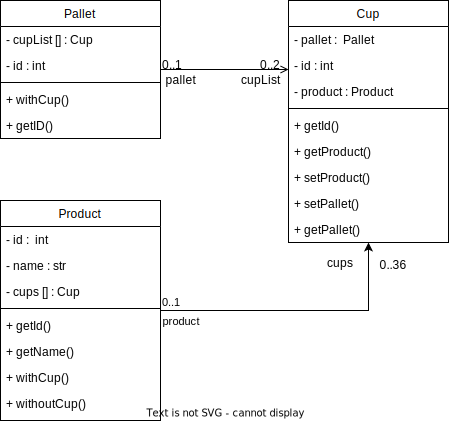
\includegraphics[width = \textwidth ]{Bilder/BeispielRefInt}
        \centering
\end{figure}

In die Klassen der Datenmodelle sollen nur Klassen gespeichert werden, die dynamisch sind. D.h. sie werden zur Laufzeit geändert und/oder
erzeugt bzw. gelöscht. 
Für die Modellierung der Daten wird das MVVC Konzept angewandt und um Serviceklassen erweitert.

Bei der Anlieferung eines Bechers wird dieser in eine Palette gestellt und anschließend eingelagert.
Ein Objektdiagramm dieser Situation ist in Abb.\ref{fig:figure14} dargestellt.

Eine Palette kann keinen, einen oder zwei Becher beinhalten.
Die Becher in einer Liste in dem Paletten-Objekt zu speichern hat den Nachteil, dass man die Becher in der Palette als Listeneinträge verarbeiten muss
und der Slot als weitere Listenspalte geführt wird.

Die Becher als zwei separate Attribute des Paletten-Objekts zu führen hat den Nachteil, dass zwei Orte abgefragt werden müssen.
Andererseits ist die Zuordnung des Bechers zum Slot dadurch inhärent.
Daher wird dieser Ansatz gewählt.

Abb. \ref{fig:figure14} zeigt auch, dass jedes Objekt der Klasse Palette und Cup ein Feld \verb|location| braucht.
Hier wird das Objekt gespeichert in dem sich die Palette oder Becher gerade befindet.

Dies ist erforderlich um referenzielle Integrität zu gewährleisten und erleichtert die Implementierung der Controller,
wie eingangs in Kapitel \ref{PythonApp} beschrieben.

Aus dem Diagramm wird auch deutlich, dass zwsichen den Objekten der Klassen \verb|MobileRobot|, \verb|WorkBench| und
\verb|Inventory| keinerlei Assoziationen gibt.

Es wird also ein weiteres Objekt, z.B. ein InventoryController, gebraucht um aktiv Objekte von einem Lagerort zu einem Anderen
zu schreiben.
Immer wenn ein Service Zugriff auf das Datenmodell braucht, wird der entsprechende Controller diese Zugriffe verarbeiten.
Als Ergebnis dieser Überlegungen leitet sich ein (Daten-)Klassendiagramm ab (Siehe Abb.\ref{fig:figure15}).

\begin{figure}
        \caption[Objektdiagramm]
        {\small Die Abbildung zeigt ein Objektidiagramm aus Ablageorten für Paletten und Becher. Es ist ebenfalls
        ersichtlich, dass keine Verbindungslinien zwischen dem mobilen Roboter, dem Kommissioniertisch und dem Lager existieren.
        }\label{fig:figure14}
        \includegraphics[width = \textwidth ]{Bilder/Objektdiagramm_PaletteCupStorage}
        \centering
\end{figure}

\begin{figure}
        \caption[Klassendiagramm Datenmodell ]
        {\small Klassendiagramm für die Datenstruktur der Software der Lagerverwaltung.
        }\label{fig:figure15}
        \includegraphics[width = \textwidth ]{Bilder/Klassendiagramm_Datenstruktur}
        \centering
\end{figure}

\subsection{Datenklassen}

In den Datenklassen sollen alle realen Objekte abgebildet werden, die durch das Lager bewegt sind oder daran aktiv/passiv beteiligt sind. 
Das betrifft: 

\begin{enumerate}
        \item Becher.
        \item Paletten, weil sie Becher beinhalten können und mit oder ohne Becher bewegt werden. 
        \item Greifer, wei er die Becher und Paletten bewegt. Ein Ausfall der Lagerzelle kann bewirken, dass ein Becher / Palette auf dem Greifer verbleibt.
        \item Kommissioniertisch, weil er Ziel von Transportbewegungen ist.
        \item mobile Roboter, weil er Quelle und Ziel von Transportbewegungen ist.
\end{enumerate}

\subsection{Konstante Daten}

Daten, die über die im Rahmen der Entwicklung festgelegt werden und sich üblicherweise nicht Ändern, sollen in einer
eigenen Klasse gespeichert werden und \verb|constants| heißen. 
Dort soll gespeichert werden: 

\begin{itemize}
        \item Dateipfade zu allen Dateien, die das Programm verwendet oder erzeugt. Dies können z.B. Konfigurationsdateien, Logdateien oder Dateien zum Abspeichern von Daten sein.
        \item Strategische Werte, die in der Entwicklung festgelegt und mehrfach verwendet werden. 
\end{itemize}

\subsection{Programmeinstellungen}

Programm-Einstellungen sollen in einer eigenen Klasse \verb|preferences| gespeichert werden.
Die Einstellungen sollen in einer Datei gespeichert werden, sobald der Benutzer eine Änderung speichert.

\section{Konzepte für Controller- und Serviceklassen}\label{ControllerServices}

Die Kommunikation über Modbus wird durch OPC UA ersetzt.
Für die Kommunikation über diese Schnittstelle wird ein \verb|OpcUaService| implementiert.

Ein Service übernimmt die Kommunikation mit den RFID-Lesegeräten in der $\mu$Plant und stellt die ausgelesenen Daten
über den \verb|OpcUaService| den anderen Stationen zur Verfügung.

Das in \cite{LarsKistner2017} eingeführte Agentensystem wird ebenfalls als eigener Service implementiert.
Da die LZ nicht mit anderen Stationen kommunizieren muss, reicht die Implementierung des Clients.
Dabei wird die Kommunikation über OPC UA realisiert.

Controller werden gebraucht um Schnittstellen zwischen Service und Daten oder zwischen Service und GUI zu implementieren.
Eine besondere Rolle nimmt der \verb|InventoryController| ein.

Er muss zum Start des Programms das Inventar aus Dateien laden und damit das Datenmodell initialisieren.
Aus Gründen die in Kapitel \ref{Fehlerbehandlung} erörtert werden, sollte der Controller nach jeder vollständigen Änderung
des Datenmodells die Änderung einerseits in der Datei sichern.

Eine Liste aller benötigter Service Klassen ist in Tab. \ref{tab:Services} aufgelistet.
Die Controller finden sich in Tab. \ref{tab:Controller}.


\begin{table}[h]
\centering
\caption{Benötigte Serviceklassen}
\begin{tabularx}{\textwidth}{|l|X|}
\hline
Klassenname & Beschreibung \\
\hline
Modbus Service & Implementiert die Modbus Kommuniktaion, sendet Modbus informationen an entsprechende Controller\\
\hline
OPC UA Service & Hält OPC UA Server und Client, organisiert Kommunikation zu anderen OPC UA entities\\
\hline
RFID Service & Erledigt alles was mit RFID zu tun hat\\
\hline
\end{tabularx}\label{tab:Services}
\end{table}


\begin{table}[h]
\centering
\caption{Werte der Klasse ModbusBaseAddress}
\begin{tabular}{|l|l|}
\hline
Klassenname & Beschreibung \\
\hline
InventoryController & Führt jede Operation bezüglich des Datenmodells aus \\
\hline
EventlogController & Erzeugt Meldungen für den Eventlog\\
\hline

\hline
\end{tabular}\label{tab:Controller}
\end{table}



\section{GUI Konzeptionierung}

Neben der Datenmodellierung und der Programmlogik ist die GUI ein wichtiger Bestandteil der Software.

\subsection{PySide6 und QuickQml 2.0}

Laut der Qt Wiki Website \cite{QtWikiHistory} wurde das Qt Framework geboren, als ihre Schöpfer Haavard Nord und
Eric Chambe-Eng im Sommer 1990 in Norwegen an einem GUI für eine Ultraschalldatenbank arbeiteten.

Die Software sollte damals in C++ implementiert auf Mac, Unix und Windows laufen.
Fünf Jahre später veröffentlichten Sie das erste Qt Framework unter dem Firmennamen Troll Tech.
Seitdem gewann das Framework immer mehr Popularität.
Im Jahr 2006 übernahm Nokia die Firma Troll Tech und verkaufte das Qt Project in den Jahren 2011 und 2012 erst teilweise,
dann vollständig an den Digia Konzern.
Seit 2014 ist Qt als Tochterunternehmen des Digia Konzerns unter dem Namen \glqq The Qt Company\grqq{} ein eigenständiges Unternehmen.

Das Qt Framework ist in C++ implementiert.
Die neue Software für die $\mu$Plant soll jedoch in Python implementiert werden.
Für diese Zwecke hat Qt u.A. das Framework PySide6 veröffentlicht, welches einen Wrapper für Python Projekte bietet.

GUI's können in PySide6 zwei Paradigmen folgend erstellt werden.

Eine Möglichkeit ist es, das GUI über Widgets\cite{pysideQtWidgets} zu erstellen.
Dabei werden GUI Elemente als eigene Klasse direkt im Python implementiert.
Dies ist eine schnelle und unkomplizierte Art einfache GUIs zu erstellen. 

Die zweite Möglichkeit ist QtQuick \cite{pysideQtQuick} zu nutzen. 
Neben der Instanz einer \verb|QGuiApplication| wird eine \verb|QQmlApplicationEngine| instanziiert.
GUI Elemente werden in einer separaten QML-Datei erstellt und mit dieser geladen und gerendert. 
Dies bietet den Vorteil, dass für das GUI eine deklarative Sprache verwendet wird, die sich von der Programmlogik trennt.
Die Bibliothek \verb|QtQuick 2.0| beinhaltet viele grundlegende QML-Datentypen, die beliebig zu GUIs kombiniert werden können.

Für die Umsetzung eines MVVC-Design Patterns empfiehlt sich die Verwendung von QML.
Durch die Verwendung des Frameworks wird die konsequente Trennung zwischen Interface und Datenmodell erzwungen.
Veranschaulicht wird dies in Abb. \ref{fig:figure10}.


Um die anwendungsspezifischen Datenmodelle (Model) in einem GUI (View) zu verwenden, muss das Datenmodell als Ressource
der \verb|QQmlApplicationEngine| zur Verfügung gestellt werden.
Zu diesem Zweck werden Klassen implementiert, die von Qt-Klassen erben, die wiederumg von \verb|QtAbstractModel| abgeleitet sind.
Die Klasse muss der Datenstruktur des Datenmodells entsprechen. In diesem Projekt sind \verb|QAbstractListModel| für Listen
und \verb|QAbstractTableModel| für tabellenartige Datenstrukturen relevant.

In diesen Klassen müssen bestimmte Methoden überschrieben werden. Manche andere Methoden sind optional. 
Welche Methoden das sind ist in der Referenzdokumentation des Qt Frameworks nachzulesen.

Die Implementierungen der Methoden ist individuell und hängt von der Datenstruktur ab. Die Datentypen der Argumente und Rückgabewerte sind 
jedoch vorgegeben.

Wenn in einem GUI z.B. eine Liste sortiert oder gefiltert werden soll, dann muss zusätzlich ein sog. \verb|QSortFilterProxyModel|
implementiert werden. 

Bevor die Instanz der \verb|QQmlApplicationEngine| die erste QML-Datei lädt - also vor Programmstart - muss entweder die Instanz des
\verb|QSortFilterProxyModel| oder die Instanz des \verb|QAbstractModel| als Ressource der \verb|QQmlApplicationEngine| registriert werden.
Diese Instanz ist dann das Viewmodel. Die Implementierten Methoden dienen dazu die Daten des Datenmodells beim Rendern zu verarbeiten. 

Über das GUI können die Daten des Viewmodels geändert, gelöscht oder hinzugefügt werden - ohne zwangsweise das Datenmodell selbst zu ändern.

Wenn ein Viewmodel mit der \verb|QQmlApplicationEngine| verknüpft ist, kann es über seine URI in jeder QML-Datei angesprochen werden.

In einer QML-Datei wird einem entsprechenden QML-Datentyp, z.B. \verb|ListView| für eine einfache Liste,
über das Property \verb|model| die URI des Datenmodells zugewiesen.
Dadurch kennt das \verb|ListView| Objekt die Indices des Datenmodells und erhält beim Rendern der Liste nur die benötigten
Daten.

Jede weitere Aktion, die durch den Benutzer auf ein Listenelement ausgelöst wird, bezieht sich auf ein Delegate des Datenmodells.
Jede Änderung an dem Delegate wird zunächst gerendert und überprüft bevor das Datenmodell geändert wird.
Diese Basisfunktion kommt mit dem Qt Framework an sich und muss nicht implementiert werden.
Wie jedoch das Datenmodell mit den geänderten Daten umgeht oder ob die Änderung des Datenmodells automatisch ein Update
der Daten auf dem Server oder der Datei auslöst, muss vom Entwickler implementiert werden!

Die Kommunikation des GUIs mit der Anwendung erfolgt über Signale und Slots.
Signale sind Teil des Signal/Slot Prinzips des Qt Framework \cite{pysideSignalSlot} und stellen die Funktion eines Events dar.
Wird ein Signal an beliebiger Stelle im GUI emittiert, kann es an jeder anderen Stelle als Event genutzt werden.
Dadurch muss man in der Regel keine zusätzlichen Callbacks oder Lamda-Ausdrücke benutzen.

Außerhalb des QML-Contexts, z.B. in einer Python Klasse, muss das Signal der Klasse bekannt sein, indem das Signal an die Klasse
gebunden wird.

Eine Funktion, die mit der Annotation \glqq @Slot()\grqq{} versehen ist, wird als Slot behandelt und kann mit dem Signal
verknüpft werden, sodass diese bei Auftreten des Signals ausgeführt werden.

Ist eine Methode einer Klasse ein Slot und ist diese Klasse als Ressource der \\\verb|QQmlApplicationEngine| registriert,
dann kann im QML-Code der Slot der Klasse auch direkt aufgerufen werden. 

An Signale und Slots können Daten übergeben werden.
Bei der Deklaration eines Signals oder Slots müssen als Argumente für jedes übergebene Datum der Datentyp angegeben werden. 
z.B.: $$@Slot(str, int)$$

Anzahl und Datentyp der Argumente müssen bei deklarierten Signalen und Slots jederzeit übereinstimmen. 
Dass Datentypen in Python dynamisch sind kann unter Umständen zum Problem werden. 
Der Datentyp \verb|None| ist im QML-Kontext nicht bekannt und führt zu einer Fehlermeldung. 
Es kann also erforderlich sein die zu übergebenen Daten auf die Datentypen zu casten oder in sinnvolle Werte umzuwandeln.

In meiner Vorbereitung auf diese Arbeit hat sich eine intuitive Vorgehensweise entwickelt, die ich für die Implementierung
der Software empfehlen möchte:

Beim Initialisieren des Programms werden alle Datenmodelle (\verb|QAbstractModel| und abgeleitete Klassen), Controller
und Serviceklassen instanziiert und als Root-context der \verb|QQmlApllicationEngine| gesetzt.
Siehe dazu das Beispiel \ref{exampleApp}.
Damit stehen sie dem Programmierer in jeder QML-Datei der Anwendung zur verfügung.

In einer QML-Datei können die Kontexte der QQmlEngine nun unter ihrer URI referenziert werden.
Dies ist in Beispiel \ref{exampleListview} gezeigt:

In dem QML-Datentyp \glqq ListView\grqq{} wird dem Property \verb|model| die URI des ListModels aus \ref{exampleApp} zugewiesen.
Im weiteren Verlauf des Codes findet sich ein \verb|MouseArea| QML-Datentyp.

Wird in dem Bereich ein Klick mit linker Maustaste durchgeführt, wird das Signal \\\verb|onClicked| emittiert.
Innerhalb des Codes im Funktionskörper der \verb|MouseArea| ist definiert, dass nach einem Mausklick die Funktion \verb|selectRow(message)|
aufgerufen wird. \verb|message| ist dabei der übergebene Parameter.

Das Beispiel braucht dabei keinerlei Importe anderer Klassen, was daran liegt, dass sowohl das DatenModell als
auch das Objekt der Controller Klasse als Ressource der QQmlEngine registriert wurden.

Im weiteren Verlauf des Codes wird ein QML-Datentyp \verb|Connections| dazu benutzt, das Signal des Controllers \verb|onRowClicked|
mit einer Funktion zu verbinden.
Die Funktion wird innerhalb des \verb|Connections|-Datentyps in JavaScript implementiert.

Gemäß der Namenskonvention ist das Signal im Controller selbst als \verb|RowClicked| deklariert!
Innerhalb der QML-Datei werden die Signale dann mit dem Präfix \glqq on\grqq{} erfasst.

Der Signalname wird als Name einer JavaScript-Funktion verwendet, die mit \verb|function| gekennzeichnet ist.
Der Code innerhalb des Funktionskörpers beschreibt dann die Funktionslogik im JavaScript-Syntax.
Im Fall des Beispiels wird ein bool'sches Property umgeschaltet, wenn die \verb|id| des Datenmodell-Delegates mit der
\verb|message| des Signals übereinstimmt.

\lstset{
    basicstyle=\small\ttfamily
}
\newpage
\lstinputlisting[language=Python,
        caption ={Beispiel einer einfachen App mittels PySide6. \small Zunächst wird eine Instanz der
Application-Klasse und der QmlEngine erzeugt. Danach werden Objekte eines Datenmodells und
eines Controllers erzeugt und als rootContext der QmlEngine registriert. Anschließend wird die QML-Datei des Hauptfensters geladen,
was die App startet.}]
{Listings/Demo1.py}\label{exampleApp}

\lstinputlisting[language=xml,
caption ={Beispiel einer QML-Datei\small Diese QML-Datei erzeugt ListView QML-Datentyp, der zum Anzeigen der Daten
in einem ListModel verwendet wird. Innerhalb eines Rechtecks mit farbigem Rand werden in einem RowLayout Type die
Datensätze des Datenmodells gerendert und über die Funktionslogik von Signalen der QML-Datentyps und der Controllerklasse
farblioch markiert.}]{Listings/listviewExample.qml}\label{exampleListview}
\newpage

\begin{figure}
        \caption[Model-View Konzept mit zusätzlichem Controller und Service ]
        {\small Die Abbildung zeigt das in PySide6 verwendete Model-View Konzept, welches um einer Controllerklasse und
        einer Service Klasse erweitert wurde. }\label{fig:figure10}
        \includegraphics[width = \textwidth ]{Bilder/MVCS_Beispiel}
        \centering
\end{figure}

\newpage

Aus den Beispielen \ref{exampleApp} und \ref{exampleListview} lässt sich eine Systematik erkennen:
Die Daten sind hinter einem ViewModel geschützt und werden der View zur Verfügung gestellt.

Über die QML-Dateien erfolgt die GUI Modellierung und Events werden mit dem Signal/Slot Prinzip behandelt.
Beliebige Ressourcen können als Teil der QmlEngine registriert werden, um Sie an anderer Stelle verfügbar zu machen.

Das künftige Programm soll jedoch auch Programmteile aufweisen, die nicht unbedingt mit den Daten oder dem GUI verknüpft sind.

Z.B. die Kommunikation über ModBus und zum ABB Industrieroboter oder das Übersetzen der Modbus Werte in
RAPID Befehle.
Diese Programmteile werden als Service Klassen bezeichnet.
Wenn sich der Programmcode auf ein GUI auswirkt, wird ein Controller gebraucht, der dieses Verhalten steuert.

Die Funktionen eines Services in den Controller zu integrieren würde die Wartbarkeit und Erweiterbarkeit verschlechtern.

Nach der Systematik wie in Abb. \ref{fig:figure10} abgebildet, können beliebig viele Datenmodelle, GUI's, Controller und Services
parallel existieren ohne sich gegenseitig zu beeinflussen.

Als Nachteil kann angeführt werden, dass sich mit zunehmendem Kontextregister der QmlEngine die Performance des Programms
verschlechtern wird.
Bei dem eher gering erwarteten Funktionsumfang der zu erstellenden Software wird dies jedoch untergeordnet behandelt und könnte
durch das Aufteilen der Funktionen in Threads reduziert werden.

\section{GUI - Modellierung}

Die Hauptfunktion der Software ist das automatisierte Abarbeiten der Kommissionsaufträge, die bisher über Modbus TCP/IP
von der Auftragsverwaltung der $\mu$Plant übergeben werden.
Während der Automatikbetrieb läuft, wird ein Benutzer allenfalls einen Soll-Ist-Vergleich zwischen dem Stand der 
Software und der realen Lagerzelle durchführen.
Die Idee ist daher, dass das neue GUI im Vergleich zum Alten aufgeräumter und übersichtlicher wird. 
Informationen die unmittelbar mit dem Prozess verbunden sind, sollen leicht ersichtlich und verfügbar sein. 
Alle anderen Informationen sollen nur bei Bedarf angezeigt werden.

In Abb. \ref{fig:figure11} zeigt meinen Entwurf zu dieser Idee:

Links ist die Andockstation des mobilen Roboters simuliert mit einem RFID Gerät darüber.
Die eingelesen Daten des RFID -Lesers könnten rechts daneben angezeigt werden, sobald der Benutzer mit der Maus 
darüber hovert. Wenn aktuell ein Tag gelesen wird, könnte das Symbol die Farbe wechseln.

Der Kommissioniertisch ist mit seinen beiden Plätzen \glqq K1\grqq{} und \glqq K2\grqq{}  daneben symbolisiert.

Die Visualisierung des Lagers nimmt die gesamte rechte Bildschirmhälfte ein.

Die Produktliste, wie sie in \ref{fig:figure} Bereich \glqq D\grqq{} dargestellt ist, ist im GUI nicht mehr vorhanden.
Muss der Bediener ein Produkt an irgendeiner Stelle des Programms überschreiben, so wird ihm nicht mehr die Produkt-ID
angezeigt, sondern direkt der Produktname.
Zusätzlich kann die Produktliste als Neues Fenster über die Toolbar eingeblendet werden.

Sämtliche Einstellungen wie IP und Port der Kommunikationsschnittstellen werden nur selten gebraucht.
Über die Toolbar sind die Einstellungen über den QML-Datentyp \verb|QDialog| einsehbar.

Eingegebene Daten müssen bestätigt werden und können auch wieder verworfen werden.

Die Bereiche \glqq E\grqq{} (Inventarliste) und \glqq F\grqq{} (Eventlog) aus Abb. \ref{fig:figure} müssen nicht
gleichzeitig sichtbar sein. 
Sie werden in einem Register integriert und mit dem QML-Datentyp \verb|StackView| oder einem Loader angezeigt.
Das Erscheinungsbild der beiden GUI Elemente kann aus der alten Software übernommen werden.
Als Drittes Register soll zusätzlich zum alten Startbildschirm eine Commission List (siehe Abb. \ref{fig:figure13}) hinzugefügt werden.
Sie soll eine Übersicht über die von der Auftragsverwaltung eingetroffenen Aufträge und ihren Status anzeigen.

Um manuelle Überschreibungen der Produkte und Becher vorzunehmen, wird statt des Checkbox-Menüs ein Zahnrad-Symbol erscheinen,
wenn man über dem entsprechenden Bereich den Mauszeiger führt (Hovering).
Mit Klick auf das Zahnrad-Symbol soll ein Objekt des QML-Datentyps \verb|QDialog| eingeblendet werden in dem die alten
Feldwerte angezeigt und editiert werden können, aber auch das Editieren verworfen werden kann.


Die Funktion des ehemaligen Controllers wird über die Toolbar aufgerufen.
Der Begriff \glqq Controller\grqq{} an sich ist im Zusammenhang mit der neu konzipierten Software irreführend und wird daher verworfen.
Der stattdessen wird der Titel \glqq Manual Processing\grqq{} gewählt.
Hiermit sollen manuell Transportaufträge erzeugt werden wie z.B. \glqq Räume den Becher aus Lagerort L3a nach L6b\grqq{}.
Dies soll für jede sinnvolle Transportoperation möglich sein.
Mit Klick auf den entsprechenden Eintrag in der Toolbar öffnet sich ein Fenster oder ein Dialog, wie in Abb.\ref{fig:figure12}.
Die so neu erzeugten Transportaufträge werden ebenfalls in der Commission List (siehe Abb. \ref{fig:figure13}) angezeigt.


\begin{figure}
        \caption[Mockup des Startbildschirms]
        {\small Die Abbildung zeigt wie der Startbildschirm aussehen könnte um die Funktion des Automatikbetriebs abzubilden:
        }\label{fig:figure11}
        \includegraphics[width = \textwidth ]{Bilder/Mockup_Startbildschirm}
        \centering
\end{figure}

\begin{figure}
        \caption[Mockup des Menüs für die manuelle Lagersteuerung]
        {\small Die Abbildung zeigt, dass entweder ein Becher oder eine Palette (mit oder ohne Becher) vom Startort zum
        Zielort transportiert werden kann. Die Eingabe der Zielorte wird hier über zwei Dropdown Menüs realisiert.
        Das Mockup impliziert, dass bei Tätigung einer Eingabe eine Validierung der Eingaben erfolgt.
        }\label{fig:figure12}
        \includegraphics[height = 0.5\textwidth ]{Bilder/Mockup_ManualProcessing}
        \centering
\end{figure}

\begin{figure}
        \caption[Mockup der Commission List]
        {\small Die Abbildung zeigt, wie die Commission List aussehen könnte. Sie könnte als Tab in einem Register eingebunden werden.:
        }\label{fig:figure13}
        \includegraphics[width = \textwidth ]{Bilder/Mockup_CommissionList}
        \centering
\end{figure}
\vspace{1cm}

Das GUI des RFID Server Programms war sinnvoll und praktisch und kann so wie bisher umgesetzt werden.
Der Aufruf des Programms soll über die Toolbar implementiert werden.

\newpage
\section{Teilautomatisierte Code Dokumentation mit Sphinx}

Code-Dokumentation ist ein wichtiger Bestandteil jedes Softwareprojekts und dient dazu den Code anderen Entwicklern zugänglich zu machen.
Die Erstellung ist unter Umständen aufwändig, kann aber zumindest teilweise automatisiert werden.
Eine Möglichkeit besteht darin, das Paket sphinx zu verwenden.

Sphinx ist ein Tool, das es Entwicklern ermöglicht, Dokumentationen in verschiedenen Formaten wie HTML, PDF und ePub
aus Kommentaren im Code des Python Projekts zu erstellen.
Dazu werden die in Python üblich Docstrings verwendet \cite{pepDocstrings}.

Das Paket kann über PyPi mit folgendem Kommando über die Eingabeaufforderung installiert werden:
\begin{lstlisting}
        pip install -U sphinx
\end{lstlisting}


Das Sphinx- Paket benutzt Themes um die Dokumentation grafisch darzustellen und zu strukturieren.
In Vorbereitung auf diese Arbeit habe ich mir das rtd-theme (Read the Docs \cite{RTD}) angeschaut und ausprobiert.
Es ist ein beliebtes Theme für Sphinx-Dokumentationen, da eine klare und übersichtliche Darstellung der Dokumentation
bietet und einfach zu verwenden ist.
Um das rtd-theme in einem Sphinx-Projekt zu verwenden, muss es zunächst installiert werden.
Dies kann über den Befehl
\begin{lstlisting}
        pip install sphinx_rtd_theme
\end{lstlisting}
erfolgen, dabei wird das Sphinx Paket auf die Version 6.4.1 angepasst.

Um Sphinx zu nutzen, muss es zunächst konfiguriert werden. Mit dem Kommando

\begin{lstlisting}[language = python]
        sphinx-quickstart
\end{lstlisting}
wird man Über die Konsole aufgefordert einige Optionen festzulegen mit denen die Dokumentation aufgesetzt wird.
Anschließend befinden sich in dem ausgewählten Ordner:
\begin{itemize}
        \item ein Makefile
        \item eine Datei \verb|modules.rst|
        \item eine Datei \verb|index.rst|
        \item eine Datei \verb|conf.py|
\end{itemize}

Die Index-Datei ist später der Einstiegspunkt.
Im RST-Format \cite{sphinxRST}kann die Seite gestaltet werden.

In der \verb|modules.rst| dagegen werden die Module aufgelistet, die dokumentiert werden sollen.
Nach der Installation des rtd-theme kann es in der Konfigurationsdatei von Sphinx aktiviert werden.
Dazu muss die Zeile \verb|html_theme = 'sphinx_rtd_theme'| in die Datei \verb|conf.py| eingefügt werden.
Sobald das Theme aktiviert ist, wird die Dokumentation nach dem build Vorgang im rtd-Theme angezeigt.

\subsection{Sphinx Erweiterungen}\label{subsec:sphinx-erweiterungen}

Erweiterungen werden nach der Installation des Pakets in der Konfigurationsdatei \verb|conf.py| aktiviert.
Im Rahmen habe ich viele Erweiterungen getestet und empfehle die nachfolgenden Erweiterungen zu verwenden. 
Die nachfolgende Zeile aktiviert alle Erweiterungen aus meiner Empfehlung. 

\begin{lstlisting}[language = python,label={lst:sphinxExt}]
extensions = [
        'sphinx.ext.autodoc',
        'sphinx.ext.viewcode',
        'sphinx_copybutton']
\end{lstlisting}

\subsubsection{Autodoc}

Autodoc wird dazu verwendet um die Docstrings im Python-Code als Dokumentationstext zu erfassen.
Damit dies funktioniert muss ein Modul in der Datei \verb|modules.rst| mit folgendem Syntax hinzugefügt werden:

\begin{lstlisting}[language = python,label={lst:sphinxAutomodule}]
.. automodule:: src.cameraApplication.cameraProcessing
        :members:
        :undoc-members:
        :show-inheritance:
\end{lstlisting}

\verb|:members:| sorgt dafür, dass alle Klassen und Funktionen des Moduls in der Dokumentation erscheinen.
Die verwendeten Docstrings wirden zusammen mit dem Namen und ggf. Argumenten und Rückgabewerten angezeigt.

\verb|:undoc-members:| sorgt dafür, dass auch Funktionen und Klassen ohne Docstrings in der Dokumentation erscheinen.
Die Klassen und Funktionen werden dann ohne Beschreibung angezeigt.

\verb|:show-inheritance:| sorgt dafür, dass die Vererbungshierarchie der Klassen angezeigt wird.
Dies ist in Verbindung mit dem Qt Framework oft hilfreich. Da viele Qt-Klassen eine große Vererbungskette haben, kann dies manchmal auch unübersichtlich werden.

Die Dateipfade der Module werden wie im Beispiel vom Makefile aus zur Python-Datei angegeben, jedoch ohne Dateierweiterung.
Docstrings in den Modulen werden direkt als HTML gerendert.
Inline-Kommentare werde nicht angezeigt.

QML-Dateien können auf diese Weise nicht gerendert werden. Um sie dennoch in der Dokumentation anzuzeigen,
habe ich sie in der Datei \verb|modules.rst| mit folgendem Syntax hinzugefügt:

\begin{lstlisting}[language = python,label={lst:sphinxQML}]
        qml.main.qml
        ------------
        
        The main QML-file creates the main application window.
        
        .. literalinclude:: src/qml/main.qml
                :language: qml
        \end{lstlisting}
Dadurch wird der gesamte Inhalt der QML Datei in der Dokumentation angezeigt.

\subsubsection{viewcode}

Um den Quellcode des Moduls in dem HTML Dokument einblenden zu können wird die Erweiterung viewcode genutzt.
Unterhalb der Modulüberschrift im HTML-Dokumentwerden zunächst alle Docstrings gerendert.
Darunter erscheint nun ein grauer Bereich, in dem Python Code mit Farbformatierung angezeigt wird.
Es werden auch andere Sprachen erkannt, jedoch gibt es leider keine Option QML Code farblich formatiert
anzuzeigen.
QML-Dateien werden im Allgemeinen von Autodoc nicht erkannt.
Die Einzige Option ist ein \verb|literalinclude| Befehl wie oben schon beschrieben.
Wie leicht zu erkennen werden Docstrings nicht erkannt und müssen daher manuell eingefügt werden.
Kommentare im JavaScript-Syntax und Properties werden farblich hervorgehoben.

\subsubsection{sphinx\_copybutton}

Diese Erweiterung fügt in Code-Blöcken der HTML-seite eine Kopier-Taste hinzu, mit denen 
z.B. Kommandozeilenbefehle in den Zwischenspeicher kopiert werden können.
Code-Blocks werden wie folgt angegeben:
\begin{lstlisting}[label={lst:sphinxCodebutton}]
        .. code-block:: bash
                pip install -r requirements.txt
\end{lstlisting}


\section{Sonstige Festlegungen}

Die zu verwendenden Farben sollen dem $mu$Plant Logo oder dem Logo der Universität Kassel entnommen werden.

\subsection{Virtual Environment}

Die Entwicklung der Software soll mit einer virtuellen Entwicklungsumgebung (venv) stattfinden.
Alle benötigten Pakete werden dort installiert.

Die installierten Pakete werden nicht in das Git Repository gepusht. Stattdessen wird mit
\begin{lstlisting}[label={lst:freezeReq}]
        pip freeze > requirements.txt
\end{lstlisting}
Eine Textdatei mit allen verwendeten Bibliotheken erstellt.
Läd sich ein Benutzer das Repository herunter, können mit dem Befehl
\begin{lstlisting}[label={lst:installReq}]
        pip install -r requirements.txt
\end{lstlisting}
alle benötigten Pakete installiert werden, sodass das Projekt lauffähig kompiliert werden kann.
Der Nachteil ist, dass es im Aufgabenbereich des Entwicklers liegt, nicht verwendete Pakete zu deinstallieren,
sodass sie später nicht unbeabsichtigter Weise installiert werden.


\subsection{Verwendete Programme }

Nachfolgend werden alle verwendeten Programme und Software aufgelistet, die zur Erstellung der Software benutzt werden
\begin{itemize}
        \item PyCharm Comunity Edition von JetBrains wird zur Editierung von Code verwendet. Das betrifft nicht nur Python Code,
        sondern auch alle anderen Sprachen und Syntaxe exklusiv QML. Sogar zur Erstellung von LaTeX Dokumenten wird
        PyCharm mit dem PlugIn TeXiFy verwendet.
        \item Qt Creator kann für alle Qt kompatiblen Programmiersprachen verwendet werden. Es beinhaltet außerdem den
        Qt Designer, mit dem QML-Dateien grafisch editiert werden können. Das Programm ist teilweise unbequem und umständlich,
        ist aber für QML in Python die beste Lösung um intuitiv Einstellungen an QML-Datentyps auszuprobieren.
        \item Visual Studio 2022 wird dazu verwendet den C\# Code der alten Software zu analysieren.
        Das PlugIn \glqq Class Designer\grqq{} wird dazu verwendet um die Projektmappen in Klassendiagramme darzustellen.
        \item Die Homepage Diagrams.net bietet eine gute Lösung um schnell Diagramme in UML und anderen Standards zu erstellen und
        in gewünschten Dateiformaten zu exportieren.
        \item Pictogramme und Symbole werden mit Adobe Illustrator erstellt.
\end{itemize}